\documentclass{standalone}
\usepackage{tikz}
\usepackage{tkz-euclide}
\begin{document}

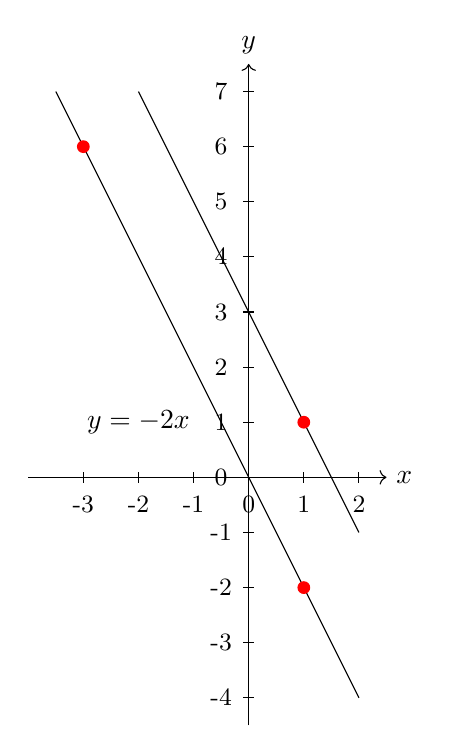
\begin{tikzpicture}[scale=0.7]
\tkzInit[xmax=2,ymax=7,xmin=-3.5,ymin=-4]
\draw [->] (0,-4.5) -- (0,7.5)node[anchor=south]{$y$};
\draw [->] (-4,0) -- (2.5,0)node[anchor=west ]{$x$};
%x-ás
\foreach \x in {-3,-2,-1,0,1,2}{
  \draw (\x,-0.5) node{\small\x};
  \draw (\x,-0.1) -- (\x,0.1);
  };
%y-ás
\foreach \x in {-4,-3,...,6,7}{
  \draw (-0.5,\x) node{\small\x};
  \draw (-0.1,\x) -- (0.1,\x);
  };

 \draw (-3.5,7) -- (2,-4) ;
 \draw (-2,7) -- (2,-1);
  \filldraw[red] (-3,6)circle(3pt);
  \filldraw[red] (1,1)circle(3pt);
  \filldraw[red] (1,-2)circle(3pt);
  \draw (-2,1) node {$y=-2x$};
\end{tikzpicture}
\end{document}
